\documentclass[a4paper,11pt]{report}
\usepackage[T1]{fontenc}
\usepackage[utf8]{inputenc}
\usepackage{lmodern}
\usepackage[spanish]{babel}
\usepackage{graphicx}
\usepackage[top=3cm, bottom=2.5cm, inner=1.5cm, outer=2.5cm]{geometry} % Márgenes personalizados
\usepackage{float} % Permite posicionar mejor las figuras y tablas
\usepackage{amsmath} % Comandos para la escritura de fórmulas matemáticas de mayor complejidad
\usepackage{amsfonts} % Proporciona fuentes matemáticas
\usepackage{amssymb} % Proporciona símbolos matemáticos de la American Mathematical Society

\title{Digit Recognizer. \\ 
  Classify handwritten digits using the famous MNIST data.\\
  Organizacion de Datos 75.06}
\author{Joaquín Blanco. Padrón 94653.\\
  Ruben Alvarado. Padrón.\\
  Diego Ripetour. Padrón.\\
  Grupo en Kaggle: The Thompsons}

\begin{document}

\maketitle
\tableofcontents
%include == include en c
%Es preferible que cada cual tenga que trabajar en su parte
%Sin tener que lidiar con el resto. A menos que así lo quiera
\chapter{Análisis Inicial de los datos.}
Previamente al diseño de la solución, se decidió realizar un análisis de los datos de entrenamiento tal que se pueda determinar sus características y formas en que las pueden ser aprovechadas.

En principio podemos decir que contamos con 42000 imágenes de 28 píxeles de ancho por 28 píxeles de alto. Cada una esta ligada a una clase de entre 10 que pueden ser 0,1,...,9. 

En la Tabla 1.1 se puede observar el porcentaje de imágenes de cada una de las clases que existen en el set de entrenamiento y como bien se puede observar, ser puede decir que el mismo esta balanceado. 

\begin{table}[htp]
  \caption{Porcentaje de imágenes de cada una de las clases en el train}
  \label{porc}

  \begin{center}
    \begin{tabular}{|c|c|c|c|c|c|c|c|c|c|c|}
    \hline
      Clase&0&1&2&3&4&5&6&7&8&9 \\
    \hline
      Porcentaje&9.83&11.15&9.94&10.35&9.69&9.03&9.85&10.47&9.67&9.97 \\
    \hline
    \end{tabular}
  \end{center}
\end{table}

Por otro lado si realizamos un promedio de todas las imágenes y observamos los valores obtenidos, daremos cuenta de que existen pixels cuyo valor es 0. Esto nos da pie para pensar que podríamos a llegar a prescindir de algunos atributos, reduciendo así el costo computacional que requerirá procesar todos estos datos. Mas adelante en el informe veremos que esto efectivamente es así.
\begin{figure}[htp]
  \begin{center}
    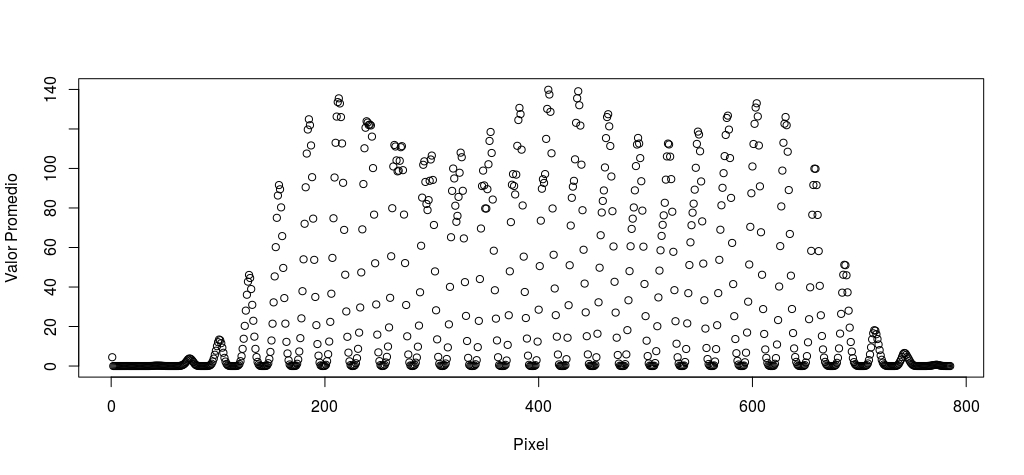
\includegraphics[width=15cm]{promImg.jpeg}
    \caption{Valores promedio de cada pixel}
    \label{promPix}
  \end{center}
\end{figure}

\chapter{Combinación de clasificadores}
La estrategia que vamos a desarrollar para cumplir con el objetivo planteado comprende llevar adelante la construcción de múltiples algoritmos de clasificación y a partir de la combinación de sus resultados lograr una mayor precisión en el reconocimiento de dígitos. En la actualidad existen múltiples estudios sobre métodos para combinar clasificadores, de entre todos ellos se decidió dar una mayor atención a aquellos que nos ofrezcan una alta precisión. Se tuvo en cuenta para la selección del tipo de combinación, los clasificadores que se van a implementar, su diversificación y su complementariedad. Cada uno de estos serán tratados mas adelante en el informe, por lo que en este capitulo nos dedicaremos exclusivamente al desarrollo de los distintos tipos de combinación que se hallaron y cual fue la elección que mejor se ajusta a nuestros objetivos e implementación.

Definiremos \textit{P} como el espacio de datos de entrada tal que $ P = C_{0}\cup...\cup C_{9} $, donde $ C_{i} $ refiere a los datos pertenecientes a la clase $ \textit{i} \in A = \{0,1,...,9\} $. Para una muestra \textit{x} extraída de \textit{P}, se puede decir que la tarea de un clasificador \textit{e} consiste en asignar un índice $ \textit{j}\in A $ a la muestra \textit{x}. Entonces \textit{e} es una función tal que $ e(x) = j  $

De acuerdo con la salida de un clasificador se definen tres tipos de problemas para los cuales se aplican distintas técnicas de combinación.
\begin{enumerate}
  \item Nivel abstracto o salida compuesta por una única clase.
  \item Nivel de rangos o listas categorizadas.
  \item Nivel de mediciones.
\end{enumerate}
Los problemas de Tipo 3 requieren que todos los clasificadores produzcan un vector de números reales de tamaño \textit{m}, siendo \textit{m} la cantidad de clases, donde en cada posición \textit{i} se guarda la probabilidad de que una muestra \textit{x} pertenezca a la clase \textit{i}. Este luego sera procesado para dotar a la muestra \textit{x} de un índice.

Por otro lado, los problemas del tipo 2 requieren que las salidas de los clasificadores sean una lista de las posibles clases a la cuales pertenezca una muestra \textit{x}. El mismo puede estar ordenada por algún criterio referente a los algoritmos que se implementaron.

Por ultimo, los problemas del tipo 1 se definen de la siguiente forma; Dados \textit{K} clasificadores individuales $ e_{k}, k = 1,...,K $ cada uno de los cuales asigna un rótulo $ j_{k} $ a una entrada \textit{x}, produciendo el evento $ e_{k}(x) = j_{k} $, se utilizan dichos eventos para construir el clasificador integrado \textit{E} que asigna $ E(x) = j $. 

Este ultimo caso admite clasificadores basados en distintas teorías y metodologías ya que solo le interesa el resultado abstracto cubriendo así todas las áreas dentro del reconocimiento de patrones. 

Es entonces que debido a su simplicidad, robustez, alta precisión en los resultados y flexibilidad que optamos por implementar métodos asociados al tipo 1. \textit{El voto por mayoría}, \textit{El voto por mayoría ponderado} o \textit{Regla de Combinación Bayesiana} son algunos de los métodos que se lograron analizar hasta el momento. De entre ellos se decidió desarrollar \textit{El voto por mayoría ponderada} dada la facilidad que comprende implementarlo\footnote{Puede que a futuro se decida cambiar esta metodología, pero por el momento se pondrá énfasis en el desarrollo de algoritmos de clasificación.}.

\section{El voto por mayoría ponderada.}
Una mejora del \textit{Voto por mayoría} consiste en considerar la confiabilidad de las respuestas de cada uno de los clasificadores individuales multiplicando cada salida por un peso. Los pesos $ w_{k} $ que expresan la competencia comparativa entre los expertos participantes, se definen como una lista de fracciones tal que
\[ \sum_{i=1}^{K}w_{i} = 1 \]
Donde \textit{K} es la cantidad de clasificadores. Cuanto mayor es la competencia de un clasificador, mayor es el valor del \textit{w} asociado.

Denotamos la desicion de un experto $ e_{k} $ que asocia una entrada \textit{x} con la clase $ i^{th} $ como $ d_{ik} $ para $ i = 0,...,9 $. La decisión que surge de la combinación de la salida de los distintos clasificadores para la clase $ i, d_{i}^{com} $, se define como:
\[ d_{i}^{com} = \sum_{k=1}^{K}w_{k} \times d_{ik} \]
La decision final $ d^{com} $ estara dada por:
\[ d^{com} = max_{i = 0,...,9} d_{i}^{com} \]

\chapter{Implementación}
Se menciono anteriormente que una de las razones por las que se desarrollo esta estrategia fue la flexibilidad con la que se cuenta, es decir, la capacidad de agregar o quietar clasificadores de acuerdo a resultados obtenidos sin la necesidad de afectar la aplicación en general. 

Una razón mas para sustentar este diseño es que se pueden obtener resultados sin la necesidad de que el costo computacional recaiga sobre un único computador. 

Si separamos el modulo encargado de combinar los resultados, de los módulos clasificadores, podremos ejecutarlos por separado. Entonces, por un lado, cada uno de los algoritmos clasificadores procesaran los datos de forma independiente del resto y generaran resultados que serán almacenados. Posteriormente, el algoritmo combinador, tomara en cuenta los resultados parciales que se obtuvieron hasta el momento de sus ejecución, los evaluara y devolverá los resultados que finalmente serán entregados a \textit{Kaggle}.

Se menciona esto para que se tenga en cuenta durante la evaluacion del trabajo realizado y el porque de su estructura.


\end{document}
